

\chapter{Introdução à Genética Quantitativa}

A genética quantiativa, em suma, é o entendimento da relação entre fenótipo e genótipo. Para isto, é necessário estudar tudo que influência esta relção.

O modelo básico para um ambiente é F = G + A. Sendo F (Fenótipo), G (Genótipo) e A (Ambiente). Para que este modelo seja aplicado a vários ambientes, é necessário adicionar outro parâmetro GA que consiste na interação entre genótipo e ambiente. Como resultado temos F = G + A + GA.

A análise do fenótipo pode ser qualitativa, como é feita na genética mendeliana, ou quantiativa como será visto ao longo do texto.


\begin{table}[h]
\centering
\begin{tabular}{l l l}
\toprule
 Fator & \textbf{Caráter Qualitativo} & \textbf{Caráter Quantitativo}\\
\midrule
 \textbf{Controle Gênico} & Poucos & Poligênica \\
\textbf{Efeito Ambiental} & Nenhum ou Pouco & Alto \\
\textbf{Distribuição dos Dados} & Discreto (Classe) & Contínuo \\
\textbf{Estado do Caráter} & (P1xP2) e Qui Quadrado & Média e Variância \\
\textbf{Interação Alélica} & Dominância completa, incompleta e codominância &  Aditiva e Não Aditiva \\
\bottomrule
\end{tabular}
\caption{Caráter qualitativo x quantitativo} \label{tab:t01}
\end{table}


Os alelos são segmentos homólogos de DNA, os alelos dominantes, são representados por letras maiúsculas, enquanto os recessivos são representados por letras minúsculas. A Interação Alélica consiste na interação ou não de genes alélicos. 

As interações alélicas qualitativas são: dominância completa, dominância incompleta e codominância. As interações alélicas quantitativas podem se dividir em aditivas: quando cada alelo contribui individualmente para o valor genotípico e consequentemente para o valor fenotípico final; não aditivas: que podem ser dominância completa, parcial ou sobredominância.

A Epstasia não é uma interação alélica, consiste em uma interação gênica.

As interações de dominância criam uma perturbação na análise quantitativa do melhoramento genético.

\section{Interação Aditiva}

Para as demonstrações assuma dois genes A: A1,A2 e B: B1, B2. Além disso vamos adimitir valores para A1,B1,A2 e B2; sendo A1 = B1 = 30 unidades e A2 = B2 = 5 unidades.

Temos:

\begin{enumerate}
\item  Parental 1 (P1): A1A1B1B1 (120 unidades)
\item  Parental 2 (P2): A2A2B2B2 (20 unidades)
\item  *P1 e P2 são puros e contrastantes
\end{enumerate}

O cruzamento entre P1 e P2 terá como resultado F1 (A1A2B1B2), realizando a autofecundação em F1, teremos F2 que poderá gerar os genótipos como mostra a tabela abaixo:



\begin{table}[h]
\centering
\begin{tabular}{l l l}
\toprule
 \textbf{Genótipos} & \textbf{Frequência} & \textbf{Valor Genotípico}\\
\midrule
 A1A1B1B1 & 1/16 & 120 \\
 A1A1B1B2 & 2/16 & 95  \\
 A1A1B2B2 & 1/16 & 70  \\
 A1A2B1B1 & 2/16 & 95  \\
 A1A2B1B2 & 4/16 & 70  \\
 A1A2B2B2 & 2/16 & 45  \\
 A2A2B1B2 & 1/16 & 70  \\
 A2A2B1B1 & 2/16 & 45  \\
 A2A2B2B2 & 1/16 & 20  \\
\bottomrule
\end{tabular}
\caption{Genótipos Possíveis em F2} \label{tab:t01}
\end{table}

Considere \ol{X} como a média aritmética de um conjunto de valores.

A média pode ser calculada utlizando a soma simples ou a frequência dos itens.

\begin{formula}[Média]
\begin{align}
& \overline{X} =  \cfrac{\sum_{1}^{n} x_i}{n} \\
\end{align}
\end{formula}

\begin{formula}[Média]
\begin{align}
& \overline{X} = \cfrac{\sum_{1}^{n} f_i\times{x_i}}{f_i}
\end{align}
\end{formula}


Utilizando os dados da tabela \ref{tab:t01}, pode-se calcular a média dos valores genotípicos de F2.


\begin{solution}[Solução do Exemplo]

\begin{align}
& \overline{X} = \cfrac{\sum_{1}^{n} f_i\times{x_i}}{f_i} \\
& \overline{X} = \cfrac{ 1\times{120} + 2\times{95}  + 2\times{70}  + 2\times{95}  + 4\times{70}  + 	2\times{45}  +  1\times{70}  +  2\times{45}  +  1\times{20} }{16} \\
& \overline{X} = 70 \\
\end{align}

\end{solution}

Quando a interação é aditiva, a médica de qualquer descendência é igual a média de seus pais. 

Segregantes transgressivos consistem em indivíduos em que seus valores genotípicos sejam maiores ou menores que seus pais. Para exemplificar, considere A1,B1,C1,D1 = 30 unidades e A2,B2,C2,D2 = 5 unidades. Considere os seguintes valores:

\begin{enumerate}
\item P1 = A1A1B1B1C2C2D2D2
\item P2 = A2A2B2B2C1C1D1D1
\item F1 = A1A2B1B2C1C1D1D2
\item F2 = Autofecundação de F1
\end{enumerate}

Dentre as 81 possibiblidades de F2, pode-se listar dois exemplos de segregantes transgressivos:

\begin{enumerate}
\item F2-1 = A1A1B1B1C1C1D1D1 = 240 unidades
\item F2-2 = A2A2B2B2C2C2D2D2 = 40
\end{enumerate}

\section{Interação de Dominância}

As interações de dominância ocorrem quando existe a relação de dominância entre alelos, ou seja, quando o alelo dominante está presente, o recessivo não contribui para a característica. Para exemplificar considere:

\begin{enumerate}
\item Gene A, sendo 'A' (Dominante) e 'a' (recessivo)
\item Gene B, sendo 'B' (Dominante) e 'b' (recessivo)
\item AA = 60 unidades
\item Aa = 60 unidades
\item aa = 10 unidades
\item BB = 60 unidades
\item Bb = 60 unidades
\item bb = 10 unidades
\end{enumerate}

Considere também os parentais P1:AABB (120 unidades) e P2:aabb (15 unidades). O cruzamento entre P1 e P2 dá origem ao descendente F1:AaBb (120). Neste caso, quando existe relação de dominância, o valor genotípico não será a média de seus parentais, podendo ser igual a um deles, como foi o caso.


\begin{table}[h]
\centering
\begin{tabular}{l l l}
\toprule
 \textbf{Genótipos} & \textbf{Frequência} & \textbf{Valor Genotípico}\\
\midrule
 AABB & 1/16 & 120 \\
 AABb & 2/16 & 120 \\
 AAbb & 1/16 & 70  \\
 AaBB & 2/16 & 120 \\
 AaBb & 4/16 & 120 \\
 Abbb & 2/16 & 70  \\
 aaBB & 1/16 & 70  \\
 aaBb & 2/16 & 70  \\
 aabb & 1/16 & 20  \\
\bottomrule
\end{tabular}
\caption{Genótipos Possíveis em F2} \label{tab:t03}
\end{table}

Com base nos dados da \ref{tab:t03} a média de F2 = 95, como a média de F1 é 120, pode-se concluir que houve a diminuição na média dos valores genotípicos. 

\begin{table}[H]
\centering
\begin{tabular}{l l l l l}
\toprule
 \textbf{X} & \textbf{AB} & \textbf{Ab} & \textbf{aB} & \textbf{ab} \\
\midrule
 \textbf{AB} & AABB & AABb & AaBB & AaBb \\
 \textbf{Ab} & AABb & AAbb & AaBb & Aabb \\
 \textbf{aB} & AaBB & AaBb & AaBB & aaBb \\
 \textbf{ab} & AaBb & Aabb & aaBb & aabb \\
 
\bottomrule
\end{tabular}
\caption{Genótipos Possíveis} \label{tab:t04}
\end{table}


\section{Grau médio de Dominância}

O grau médio de dominância mede a posição relativa do heterozigoto em relação à média dos homozigotos. 

\begin{figure}[h]
  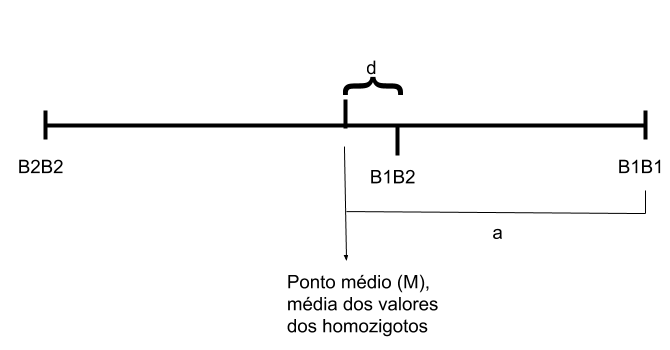
\includegraphics[width=0.9\linewidth]{img/grau-medio-dominancia.png}
  \caption{Grau Médio de Dominância}
  \label{fig:boat1}
\end{figure}


O valor do grau médio de dominância pode ser obtido dividindo-se d por a, esses valores são apresentados na \ref{fig:boat1}.


\begin{table}[H]
\centering
\begin{tabular}{l l }
\toprule
 \textbf{Resultado da Divisão} & \textbf{Interação Intra Alélica} \\
\midrule
 d/a = 0     & Interação  Aditiva  \\
 d/a = 1     & Dominância Completa \\
 0 < d/a < 1 & Dominância Parcial  \\
 d/a > 1     & Sobredominância     \\
\bottomrule
\end{tabular}
\caption{Genótipos Possíveis} \label{tab:t04}
\end{table}

O efeito de dominância mascara o processo de seleção, pois, ele dificulta o conhecimento dos indivíduos superiores pelos efeitos aditivos.

\section{Caráter Quantitativo}

O modelo para o estudo do caráter quantitativo é:

\begin{formula}[Fórmula Geral]
F = G + A
\end{formula}

\begin{definition}
Considere V(X) como a variância de X e Cov(X) como a covariância de X.

\begin{equation}
V(F) = V(G+A) \rightarrow V(F) = V(G) + V(A) + 2\times Cov(G+A)
\end{equation}

Como:

\begin{equation}
Cov(G+A) = 0
\end{equation}

Temos: 

\begin{equation}
V(F) = F(G+A) \rightarrow V(F) = V(G) + V(A) 
\end{equation}

\end{definition}





A variância (V) é descrita pela seguinte fórmula: 

\begin{formula}
\begin{equation}
V(F) = \cfrac{\sum_{1}^{n} (x_i - \overline{X})^2}{n-1}
\end{equation}
\end{formula}
ou

\begin{formula}
\begin{equation}
V(F) = \cfrac{\sum_{1}^{n} x^2 - [\sum_{1}^{n} x]^2}{n-1}
\end{equation}
\end{formula}


Para o cálculo da dedução da variância ambiental, considere um gene A, com dois alelos 'A' e 'a'.


\begin{table}[H]
\centering
\begin{tabular}{l l l l l}
\toprule
 \textbf{Genótipos} & \textbf{Nº Indivíduos} & \textbf{Frequência} & \textbf{Valor Genotípico} & \textbf{Val. Gen. Codificado} \\
\midrule
 AA & n1 & n1/n = D & X1 = u + a & a  \\
 Aa & n2 & n2/n = H & X2 = u + d & d  \\
 aa & n3 & n3/n = R & X3 = u - a & -a \\
\bottomrule
\end{tabular}
\caption{Dedução} \label{tab:t05}
\end{table}

Aplicando a fórmula da média na média genotípica:


\begin{definition}[Média Genotípica]
\begin{align}
&  Mg = \cfrac{\sum_{1}^{n} f_i\times{x_i}}{f_i} \\
&  Mg = D\times a + H\times d + R \times -a \\
&  Mg  = a \times (D-R) + H\times d \\
&  Mg = u + a\times(D-R) + H\times d
\end{align}
\end{definition}


\subsection{Variância Genética}

\begin{equation}
Va(x) = (\sum_{1}^{n} x_i^2) - (\sum_{1}^{n} f_i\times x_i)^2
\end{equation}

\begin{equation}
V(G) = D \times a^2 + H \times d^2 + R \times (-a)^2 - [a \times (D - R) + H \times d]^2
\end{equation}

\subsection{Estudo do Caráter}

Para o estudo do caráter, considere:

\begin{enumerate}
\item P1: AA
\item P2: aa
\item F1: Aa (P1xP2)
\item F2: [AA,Aa,aa]
\end{enumerate}


 
\begin{definition}[Análise de P1]

\begin{align}
&  Mg(P1) = u + a \times (D-R) + H \times d\\
&  Mg(P1) = u + a \times (1-0) + 0 \times d\\
&  Mg(P1) = u + a \\
\end{align}
\end{definition}

\begin{definition}[Variância de P1]

\begin{align}
&  V(P1) = D\times a^2 + H \times d^2 + R \times (-a)^2 - [ a \times (D-R) + H \times d ]^2 \\
&  V(P1) = 1\times a^2 + 0 \times d^2 + 0 \times (-a)^2 - [ a \times (1-0) + 0 \times d ]^2 \\
&  V(P1) = 1\times a^2 + -  1\times a^2 \\
&  V(P1) = 0
\end{align}

Portanto, como só existe um genótipo possível, não existe variância. A análise de P2 utiliza o mesmo método de P1, portanto, não há variância em P2.
\end{definition}


\begin{definition}[Análise de F2]

\begin{align}
&  Mg(F2) = u + a \times (\frac{1}{4}- \frac{1}{4}) + \frac{1}{2} \times d\\
&  Mg(F2) = u + \frac{1}{2} \times d\\
\end{align}
\end{definition}


\begin{definition}[Variância de F2]

\begin{align}
&  V(F2) = D\times a^2 + H \times d^2 + R \times (-a)^2 - [ a \times (D-R) + H \times d ]^2 \\
&  V(F2) = \frac{1}{4}\times a^2 + \frac{1}{2}\times d^2 + \frac{1}{4} \times (-a)^2 - [ a \times (\frac{1}{4}- \frac{1}{4}) + \frac{1}{2} \times d ]^2 \\
&  V(F2) = \frac{1}{4}\times a^2 + \frac{1}{2}\times d^2 + \frac{1}{4} \times (a)^2 - [ \frac{1}{2} \times d ]^2 \\
&  V(F2) = \frac{1}{2}\times a^2 + \frac{1}{2}\times d^2 - \frac{1}{4} \times d^2 \\
&  V(F2) = \frac{1}{2}\times a^2 + \frac{1}{4} \times d^2 \\
\end{align}
\end{definition}


\subsection{Variância Ambiental}

\begin{definition}[Fórmulas mais utilizadas]

\begin{align}
&  V(Amb) = V(P1) \\
&  V(Amb) = V(P2) \\
&  V(Amb) = V(F1) \\
&  V(Amb) = \frac{V(P1) + V(P2)}{2} \\
&  V(Amb) = \frac{V(P1) + V(P2) + V(F1)}{2} \\
&  V(Amb) = \frac{V(P1) + V(P2) + 2 \times V(F1)}{4} \\
\end{align}
\end{definition}


\section{Herdabilidade}

A herdabilidade é um coeficiente que expressa a relação entre a variância genotípica e a variância fenotípica, ou seja, mede o nível da correspondência entre o fenótipo e o valor genético. 

\begin{definition}[Dedução de Herdabilidade]

\begin{align}
&  r = \frac{Cov(x,y)}{\sqrt{v(x) \times v(y)}} \\
&  r(F,G) = \frac{Cov(F,G)}{\sqrt{v(F) \times v(G)}} \\
&  r(F,G) = \frac{Cov(G+A,G)}{\sqrt{v(F) \times v(G)}} \\
&  r(F,G) = \frac{Cov(G,G) + Cov(G,A)}{\sqrt{v(F) \times v(G)}} \\
&  Como: Cov(G,A) = 0 \\
&  \rightarrow r(F,G) = \frac{Cov(G,G)}{\sqrt{v(F) \times v(G)}} \\
&  Como: Cov(X,X) = V(X) \\
&  \rightarrow r(F,G) = \frac{V(G)}{\sqrt{v(F) \times v(G)}} \\
&  r(F,G) = \sqrt{\frac{[V(G)]^2}{v(F) \times v(G)}} \\
&  r(F,G) = \sqrt{\frac{[V(G)]}{v(F)}} \\
&  Como: H = \frac{[V(G)]}{v(F)} \\
&  \rightarrow  r(F,G) = \sqrt{H^2} \\
\end{align}
\end{definition}


\begin{definition}[Fórmula da Herdabilidade]

\begin{align}
&  H^2 = \frac{V(G)}{V(F)} \\
\end{align}
\end{definition}

O valor da herdabilidade pode variar entre 0 e 1. Por definição, quando o valor da herdabilidade é maior que 0,7 é considerado alto para plantas. Em caso de animas, pode variar entre 0,3 e 0,4.



\subsection{Ganho de Seleção}

\begin{definition}[Fórmula do Ganho de Seleção (GS)]

\begin{align}
& GS = H^2 \times (\overline{X}_s - \overline{X}_0) \\
\end{align}
Sendo Xs a média dos indivíduos selecionados e X0 a média inicial dos indivíduos.
\end{definition}


\subsection{Média Predita}

\begin{definition}[Fórmula Média Predita (Xm)]

\begin{align}
& Xm = GS + \overline{X}_0 \\
\end{align}
\end{definition}


\subsection{Número de Genes}


\begin{definition}[Fórmula Número de Genes (Nrg)]

\begin{align}
& Nrg = \frac{(\overline{P_1} - \overline{P_2})^2}{8 \times V(G)_{F1}} \\
\end{align}
Sendo P1 a média dos parentais 1 e  P2 a média dos parentais 2 
\end{definition}

\subsection{Exemplo}



\begin{example}

Considere os dados das apresentados abaixo para resolução das questões.

\begin{table}[h]
\centering
\begin{tabular}{l l l l l}
\toprule
 \multicolumn{5}{c}{Dados Pai 1}\\
\midrule
13,13 &  20,35 & 21,60 & 17,77 & 15,74 \\
19,90 &  24,92 & 16,81 & 22,91 & 15,68 \\
19,05 &  19,30 & 20,78 & 20,64 & 15,46 \\
17,14 &  19,21 & 15,45 & 17,88 & 18,43 \\
\end{tabular}
\caption{Valores Fenotípicos} \label{tab:t06}
\end{table}


\begin{table}[h]
\centering
\begin{tabular}{l l l l l}
\toprule
 \multicolumn{5}{c}{Dados Pai 2}\\
\midrule
103,39 &  100,94 &  99,26  &  104,13 &  97,54  \\
96,24  &  106,47 &  105,45 &  95,40  &  104,52 \\
97,60  &  95,36  &  98,85  &  98,89  &  98,13  \\
98,56  &  100,37 &  105,99 &  104,95 &  98,85  \\
\end{tabular}
\caption{Valores Fenotípicos} \label{tab:t07}
\end{table}



\begin{enumerate}
\item Média P1 = 18,6075
\item Média P2 = 100,5445
\item Média F1 = 15,7740
\item Média F2 = 60,1949
\end{enumerate}

\end{example}

Questões:

\begin{enumerate}
\item Calcule a média fenotípica de P1, P2, F1 e F2;
\item Calcule a variância Fenotípica de P1, P2, F1 e F2;
\item Calcule a variância Genética de P1, P2, F1 e F2;
\item Calcule a herdabilidade e interprete o resultado;
\item Calcule o número de genes;
\item Calcule o ganho de seleção ao selecionar os 10\% melhores;
\item Calcule a heterose e heterobeltiose;
\end{enumerate}

\begin{solution} [Média de P1, P2, F1 e F2]

Para calcular a média, deve-se utilizar a fórmula da média aritmética por soma de valores:

\begin{equation}
\overline{X} =  \cfrac{\sum_{1}^{n} x_i}{n}
\end{equation}

Assim, obtemos como resultado:

\begin{equation}
\overline{P1} =  18,6075 
\end{equation}
\begin{equation}
\overline{P2} =  100,5445 
\end{equation}
\begin{equation}
\overline{F1} =  15,7740 
\end{equation}
\begin{equation}
\overline{F2} =  60,1949
\end{equation}

\end{solution}

\begin{solution} [Variância Fenotípica de P1, P2, F1 e F2]



Para calcular a variância, deve-se utilizar a fórmula da média aritmética por soma de valores:

\begin{equation}
V(F) = \cfrac{\sum_{1}^{n} x^2 - \cfrac{[\sum_{1}^{n} x]^2}{n}}{n_1}
\end{equation}

Assim, obtemos como resultado:

\begin{equation}
V(P1) =  8,1699
\end{equation}
\begin{equation}
V(P2) =  13,4026
\end{equation}
\begin{equation}
V(F1) =  15,7740 
\end{equation}
\begin{equation}
V(F2) =  45,1901
\end{equation}

\end{solution}

\begin{solution} [Variância Genética de P1, P2, F1 e F2]



Como P1 e P2 são puros, não possuem variância genética. Filhos de pais puros, também não possuem variância. Logo, Vg(P1) = Vg(P2) = Vg(F1) = 0.

Para calcular a variância genética de F2, é necessário utilizar a fórmula:


\begin{multline}
	Vg(F2) = Vf(F2) - V(amb) \\
\end{multline}

Para isto vamos calcular a Variância Ambiental:

\begin{multline}
	V(amb) = \cfrac{8,1694 + 13,4026 + 2 \times 15,7740}{4} \\
	V(amb) = 13,2801
\end{multline}

Então, temos:

\begin{multline}
	Vg(F2) = 45,1901 - 13,2801
	V(amb) = 31,91
\end{multline}

\end{solution}

\begin{solution} [Herdabilidade]


Para calcular a herdabilidade, é necessário utilizar a fórmula:

\begin{multline}
	H^2 = \frac{V(G)}{V(F)} \\
	H^2 = \frac{31,91}{45,1901} \\
	H^2 = 0,707 \\	
\end{multline}

Portanto, 70,7\% das alterações estão relacionadas aos genes. Por definição, pode-se concluir que é um valor alto.

\end{solution}


\begin{solution} [Número do Genes]

Para calcular o número de genes, é necessário utilizar a fórumula:

\begin{multline}
	Nrg = \frac{(\overline{P_1} - \overline{P_2})^2}{8 \times V(G)_{F1}} \\
	Nrg = \frac{(18,6075 - 100,5445)^2}{8 \times 31,91} \\
	Nrg = 27 genes
\end{multline}

\end{solution}



\begin{solution} [Ganho de Seleção]

Para calcular o número de genes, primeiramente deve-se calcular a média fenotípica dos 10\% melhores indivíudos (Xs), após este cálculo, pode-se utilizar a fórumula:

\begin{multline}
 GS = H^2 \times (\overline{X}_s - \overline{X}_0) \\
 GS = 0,707 \times (73,0035 - 60,1949) \\
 GS = 9,044
\end{multline}

\end{solution}


\begin{solution} [Média Predita]

Para calcular a média predita pode-se utilizar a fórumula:

\begin{multline}
 \overline{X_m} = \overline{X_0} + GS \\
 \overline{X_m} = 60,1949 + 9,04 \\
 \overline{X_m} = 69,2394
\end{multline}

\end{solution}


\begin{solution} [Heterose e Heterobeltiose]

Para calcular a heterose pode-se utilizar a fórumula:

\begin{multline}
 h = \overline{F_1} - \frac{\overline{P1} + \overline{P2}}{2}  \\
 h = 69,2710 - \frac{18,6075+100,5445}{2} \\
 h = 9,695 \\
\end{multline}

Para calcular a heterobeltiose pode-se utilizar a fórumula:

\begin{multline}
 h_b = \overline{F_1} - \overline{Melhor Pai}  \\
 h_b = 69,2710 - 100,5445 \\
 h_b = -31,2735 \\
\end{multline}

Nota: Heterobeltiose consiste na superioridade do híbrido em relação ao progenitor de melhor desempenho. Heterose, consiste no vigor híbrido, de tal maneira que o F1 híbrido destaca-se favoravelmente dos pais homozigotos com relação a um ou mais caracteres desejados.

\end{solution}
